\documentclass{article}
\usepackage{amsmath}
\usepackage[noend]{libHO/distribalgo}
\usepackage{algorithm}
\usepackage{amssymb}
\usepackage{listings}
\usepackage{amsthm}
\usepackage{dsfont}
\usepackage{stmaryrd}
\usepackage[left=2cm, right=2cm, top=2cm]{geometry}
\usepackage[utf8]{inputenc}
\usepackage{pdfpages}


\newtheorem{lemma}{Lemma}[section]
\newtheorem{theorem}{Theorem}
\newtheorem{definition}{Definition}
\usepackage{biblatex}
\addbibresource{rapport.bib}

\newcommand{\cent}{\gamma}

\newcommand{\dG}{\mathds{G}}
\newcommand{\IN}{\mathds{N}}
\newcommand{\IS}{\mathds{S}}

\newcommand{\In}{\mathrm{In}}
\newcommand{\ts}{s}
\newcommand{\tf}{\phi}
\newcommand{\try}{\tau}
\newcommand{\SM}{{\em SynchMod}$_{\,k}\ $}

\title{The $\mathrm{mod}\,k$-synchronization Problem}
\date{August 2020}
\author{Louis Penet de Monterno - Bernadette Charron-Bost}

\begin{document}

\maketitle

\section{Introduction}

The topic of distributed systems has focused a lot of attention in recent years.
Lots of today's digital services relies on distributed systems to improve the resilience of critical infrastructures.
A typical problem in distributed computing consists in emulating a data structure (stack, dictionary ...), or an algorithm (consensus ...) on a distributed
set of machines, such that the correctness of the considered algorithm is unaffected by the failures of some components.

There are two major frameworks in this field: synchronous and asynchronous systems (the exact definition of these terms may vary).
In an \emph{asynchronous system}, the model considers each machine as an individual state machine, which may progress independently from the others,
just like people working from home and communicating by email.
% They can send messages and check  to other machines whenever they want.
In opposition, a \emph{synchronous model} assumes the existence of a global schedule of execution.
The timeline is composed in a succession of rounds, the nodes make progress step by step \cite{closed_communic},
just like people having a meeting every day.
This document is focused on synchronous systems.

% In the framework of synchronous system, an assumption can be made

\subsection{Motivation}

In the literature, most of the proposed algorithms for synchronous system make an additional assumption.
This assumption tells that there exists a round at which every node starts the execution of the algorithm.
In this context, the system is said to have \emph{synchronous starts}.
In opposition, a system where each node may start at an unpredictable round is said to have \emph{asynchronous starts}.
Since most system in the literature rely on the assumption of synchronous starts, we may wonder whether this hypothesis may be avoided.

This work may be useful in practice, since the hypothesis of synchronous starts adds an engineering constraint, which in some cases is difficult to solve.
For example, let's assume that a system needs to execute several tasks in series.
When a node ends a task, he has to start the next one, however it does not know if others nodes have finished the previous task and are ready to go on.
If each task is computed with an asynchronous-starts-tolerant algorithm, that is no longer an issue.

In a system with \textit{asynchronous starts}, we suppose that initially, the nodes are not ready to execute a given algorithm. They stay passive with regard to the target algorithm, 
and signal their non-readiness by sending a special message noted null. Each node may eventually get ready in an unpredictable round of the execution.
Then, they stop sending null, and instead interact according to the code of algorithm they are executing.

\subsection{A previous proposition, and its shortcomings}

In the literature, an algorithm has been designed to simulate synchronous starts in an asynchronous-starts context.
This algorithm, named "firing squad" algorithm, can be started asynchronously in a distributed system.
Each node executing this algorithm is guaranteed to eventually raise a flag (i.e. this node is said to \textit{fire}, hence the name of the algorithm), and every node must fire in the same round.
This firing can be used as a starting signal for any subsequent non-asynchronous-starts tolerant algorithm.
This algorithm is said to solve the \textit{synchronization problem}.

However, one of the main result of this work shows that this is only doable when the communication graph is strongly connected in every round.
This required hypothesis is not compatible with crash-failures, since a crashed node must be unable to send any message.
The goal of this article is to find a solution compatible with a wider notion of fault-tolerance.

\subsection{Synchronization, consensus and failures}

The idea to solve this problem consist in weakening the specification of the synchronization problem.
During this work, we considered the following modification:
instead of requiring that every node eventually fire during the same round, we consider the subset of \textit{correct nodes}, which never crash, and whose outgoing messages are never lost.
Every node, in this subset only, is now required to fire.
In this context, the firing squad algorithm can solve the synchronization problem in spite of an arbitrary number of failures.
This adaptation of the firing squad algorithm is presented in the appendix.
However, we thought that this solution was not satisfactory. In this framework, simple send omissions have to be considered as definitive crash failure.
We want a solution which can smartly handle all kind of failures.
We tried to figure out a other way to weaken the synchronization problem.
In the next section, we describe the approach we actually chose.

\subsection{Approach of this article}

The main issue that makes existing algorithms non-asynchronous-start-resilient lies in their structure:
they are composed of several alternating phases.
For example, the well-known Paxos \cite{paxos} algorithm is structured as a rotation of four phases, (named prepare,
promise, accept, accepted).
The algorithm is supposed to work properly if each phase is executed simultaneously by every nodes.

In the case of synchronous starts, the nodes always start with the first phase (prepare), and then rotate.
In that situation, the simultaneousness of each phase is guaranteed.
However, in the case of asynchronous starts, that could result in conflicting phases executed simultaneously.

To solve this problem, we need to make sure that the starting round of each node are congruent modulo $k$,
where $k$ is a parameter representing the number of phases of the target algorithm ($k=4$ in the case of Paxos).
This problem is named \emph{$\mathrm{mod}\,k$-synchronization problem}.
The point of this article is to solve this problem.

\subsection{Proposed solution}

The goal of this document is to propose an algorithm that solves the $\mathrm{mod}\,k$-synchronization problem.
Such an algorithm could be executed on a distributed system without synchronous starts,
an at a certain round, each node would fire.
That would be a starting signal for the subsequent algorithm.
The starting signals will have to satisfy the following properties:
\begin{description}
	\item[Safety:] The starting round of each node are congruent modulo $k$.
	\item[Liveness:] Every node eventually fires.
\end{description}

\subsection{Validity domain}

We would like to maximize the fault-tolerance of our systems.
In the literature, the fault-tolerance is often expressed by the maximum number of crash-failure that are expected to happen.
Hence, a $t$-resilient system is correct if at most $t$ nodes stop working.
In the Heard-Of model \cite{CBS09} which we use, the crash-failures are not defined as a "first-class" notion.
Instead, they they can be encapsulated inside the communication assumptions.
In this article, we will consider scenarios where at least one node is able to communicate with every other node (including with itself, which is an obvious but important assumption).
This assumption is compliant with a failure of $n-1$ nodes, where $n$ is the total number of nodes.
Thus, this work is hopefully useful for real-life system.

\section{ Preliminaries}\label{sec:model}
 
\subsection{The computational model}
	
We consider a networked system with a {\em fixed} set $V$ of $n$ nodes.
We assume a round-based computational model  in the spirit of the Heard-Of model~\cite{CBS09}, 
	in which point-to-point communications are organized into \emph{synchronized rounds}: 
	each node can send messages  to all nodes and can receive messages sent  by some of the nodes.
Rounds are communication closed in the sense that no node receives messages in round~$t$ that are sent 
	in a round different from~$t$. 
The collection of \emph{possible} communications (which nodes can communicate to which nodes) at each round $t$
	is modelled by a directed graph (digraph, for short) with a set of nodes equal to~$V$.
The digraph at round~$t$ is  denoted $\dG(t)=(V,E_t)$, and is called the \emph{communication graph at round}~$t$. 
The set of $u$'s incoming neighbors in the digraph $\dG(t)$ is denoted by $\In_u(t)$.

We assume a self-loop at each node in all these digraphs  since every node can communicate with 
	itself instantaneously.	
The sequence of such digraphs~$\dG=\left (\dG(t) \right )_{t\in\IN}$ is called a {\em dynamic graph}~\cite{CFQS12:TVG}. 

In round $t$ ($t = 1, 2 , \ldots $), each node~$ u $ successively
	(a) broadcasts  messages determined by its state at the beginning of round~$ t $
	(b) receives \emph{some} of the messages sent to it,
	and finally (c) undergoes an internal transition to a new state.
A  \emph{local algorithm} for a node corresponds to a pair of
	a \emph{sending function} that determines the messages to be sent in step~(a)
	and a \emph{transition function} for state updates in step (c).
An \emph{algorithm} for the set of nodes~$V$ is a collection of local algorithms, one per node.

We also introduce the notion of  \emph{start schedules}
	that are collections~$\IS= \left (s_u \right )_{u \in V}$,
	where each~$s_u$ is  a positive integer or is equal to $\infty$.

	
The execution of the algorithm $ A $  with the dynamic graph $\dG$ and the start schedule $\IS$ then proceeds
	as follows:
Each node~$u$ is initially  \emph{passive}. 
If $s_u = \infty$, then  the node~$u$ remains passive forever.
Otherwise, $s_u $ is a positive integer, and $u$ becomes {\em active} 
	at the beginning of round~$s_u$, sets up its local variables.
In  round~$t$ $(t = 1,2\dots)$, a passive  node
	sends only heartbeats, corresponding to  \emph{null} messages,  and  cannot change its state. 	
An active node 	applies its sending function in~$A$ to its current state to generate the message to be sent to all nodes,
	then it receives the messages sent by its incoming neighbors in the directed graph~$\dG(t)$, and finally 
	applies its transition function ${\cal T}_u$ in~$A$ to its current state and the list of messages it has just received,
	(including the null messages from passive nodes) to go to  a next state. 
Since each local algorithm is deterministic, an execution of the algorithm~$A$  is entirely determined 
	by the initial state of the network,  the dynamic graph $\dG$,
	and  the  start schedule~$\IS$.
	
The states ``passive'' and ``active'' do not refer to any physical notion, and are relative to the algorithm under consideration:
	as an example, if two algorithms $A$ and $B$ are sequentially executed according to the order ``$A$ followed by $B$'',
	then at some round, a node may be active w.r.t. $A$ while it is passive w.r.t. $B$.
In such a situation, the node  is integrally part of the system and can send messages, but  these messages are empty 
	with respect to the semantics of~$B$.
	
\subsection{Network model and start model}

A \emph{network model} is any non-empty set of dynamic graphs with a permanent self-loop at each node.
We will focus on the specific network model of \emph{centered} dynamic graphs~$\dG$ defined as follows: 
	there exists some node~$\cent$ in $V$ such that every digraph $\dG(t)$ has a spanning star centered 
	at~$\cent$, i.e., 
	$$\exists \cent \in V, \, \forall u \in V, \, \forall t \in \mathds{N}, \ \cent \in \In_u(t) .$$
Note that there may be several fixed centers for~$\dG$.

As demonstrated in~\cite{CBS09}, centered dynamic graphs in the Heard-Of model captures the
	classical model of synchronous systems with a (fixed) complete communication graph and 
	 at most $n-1$ faulty senders, including the case of crashes.

Similarly, we define a \emph{start model} as a non-empty set of start schedules.
A start schedule $\IS = (s_u)_{u\in V}$ is \emph{complete} if every $s_u$ is finite, i.e.,
	no node is passive forever, yielding the model of complete start schedules.
Synchronous starts correspond to complete start schedules $\IS = (s_u)_{u\in V}$ with
	equal start rounds.	
The property of synchronous starts can be relaxed into \emph{$\mathrm{mod}\,k$-synchronous starts},
	where $k$ is any positive integer: for every pair of nodes~$u$ and $v$, it holds that $s_u \equiv s_v \!\mod k$.

\section{The \SM algorithm}

In the \SM algorithm, each node  maintains a local clock modulo $k$ with values in $\{ \overline{1}, \dots,  \overline{k} \}$.
It fires in the first round at which all the local clocks it has just heard of  are all equal to~$\overline{k} $ (line~\ref{line:fire}).
The first time a node receives discrepant clocks from its neighbors, it tries to force firing  by setting its clock to  $\overline{k} $
	(lines~\ref{line:try}-\ref{line:try+1});
	thereafter, that  just leads it to roll back its clock to 1 (line~\ref{line:tried}).
Otherwise, it receives agreed values with its own clock and then increments it by one modulo $k$ (line~\ref{line:agreed}).
Let us again stress on the fact that at each round~$t$, every active node receives the value of its local clock.
The pseudo-code of the local code of the agent~$u$ is given in Algorithm~1.

As we will see below, the difficult point in the correctness proof of the \SM algorithm is liveness.
However, right now, let us point out some properties of the algorithm that enable liveness.
First, if all the nodes  agree on the same value for their local clocks 
	-- in which case the system will be said to be \emph{monovalent} -- and if they are all active, 
	then the system remains monovalent forever.
Moreover, the common value of the local clocks is incremented by one at every later round and thus eventually 
	reaches the value~$\overline{k} $ (cf. Lemma \ref{lem:mono_liv}).
The key point of the algorithm and of its ``forced firing procedure'' lies in the fact that if all the communication graphs  
	contain a star centered at~$\cent$, then when  $\cent$ is active, its local clock necessarily becomes equal 
	to~$\overline{k}$, and every active node will eventually fire. 

% \textbf{Note:} The definition of an execution requires that a passive node always sends null. The algorithm itself requires that, at the round of its activation, a node always sends $\bot$.
% This is designed such that node just activated does not disturb a monovalent configuration with an initial value in $\mathds{Z}/k\mathds{Z}$.

\begin{algorithm}[htb]\label{algo:code}
\begin{distribalgo}[1]
\BLANK \INDENT{\textbf{Initialization:}}
	\STATE $\overline{c}_u \in \mathds{Z}/k\mathds{Z} \cup \{\bot\}$, initially $\bot$
	\STATE $tried_u \leftarrow false$
	\STATE $fired_u \leftarrow false$

\ENDINDENT \BLANK

\INDENT{\textbf{In each round $t$:}}
	\STATE send $\langle \overline{c}_u \rangle$ to all 
	\STATE receive incoming messages
	\IF{all the received messages are equal to $\overline{k}$ and $\neg fired_u$ }
		\STATE $fired_u \leftarrow true$ \label{line:fire}
	\ENDIF
	\IF{the received messages other than $null $ and $\bot$ are all equal to $i \in \{ \overline{1}, \dots, \overline{k} \}$ }
		\STATE $\overline{c}_u \leftarrow \overline{i+1} $ \label{line:agreed}
	\ELSE \IF{$\neg tried_u $ and no received message is $\overline{k}$ }
		\STATE $\overline{c}_u \leftarrow \overline{k} $  \label{line:try}
		\STATE $tried_u \leftarrow true$   \label{line:try+1}
	\ELSE
		\STATE $\overline{c}_u \leftarrow \overline{1}$ \label{line:tried}
	\ENDIF
	\ENDIF
\ENDINDENT 

\caption{The \SM algorithm} \label{algo:R}
\end{distribalgo}

\end{algorithm}


\subsection{Notation and preliminary lemmas}

In the rest of this section, we fix an execution $\sigma$ of the \SM algorithm associated to a complete activation 
	schedule~${\cal A}$ and a centered dynamic graph~$\dG \in {\cal G}^c$. % a definir 
Let $s^{\max} = \max_{u \in \Pi} s(u) < \infty$ and let~$\cent$ denote one center of~$\dG$.	


For the correctness proof of \SM, we now introduce some additional definitions.
Let $S$ be any subset of $ \mathds{Z}/k\mathds{Z}$.
Round~$t$ in~$\sigma$  is said to be \emph{$S$-valent}  if $S$ is the set of the clock values of active nodes 
	at the end of round~$t$, i.e.,
	$$ S = \{ \overline{i}  \in \mathds{Z}/k\mathds{Z} : \exists u \in \mathcal{A}_t, \ \overline{c}_u (t) = \overline{ i }\,  \}  . $$
The system is said to be $\overline{i}$-\emph{monovalent}  if the system is $\{ \overline{i}\}$-valent.

Let us define $\tf (u)$ to be the round number at which the node~$u$ fires, if any, and let $\tf(u) = \infty$ otherwise.
Similarly, let us define $\try (u)$ to be  the round number at which the node~$u$ tries to force firing
	(line~\ref{line:try}) if any, and let $\try (u)= 0$ otherwise.
It follows that $\try^{\max} =  \max_{u \in \Pi}  \try(u) < \infty$.

In the \SM algorithm, the state of each node $u$ is composed of three variables named $\overline{c}_u$, $fired_u$ and $tried_u$.
For any round $r$, we denote $\overline{c}_u(r)$, $fired_u(r)$ and $tried_u(r)$ respectively the values of these variables in the execution $\sigma$.

\begin{lemma}\label{lem:k_mono}
If $\overline{c}_\cent(t) = \overline{k} $, then the round~$t +1$  is $\overline{1}$-monovalent.
\end{lemma}
\begin{proof}
If $\overline{c}_\cent(t) = \overline{k} $, then the node $\cent$ sends $\overline{k}$ to all nodes in round $t+1$.
Hence, any active node $u$ at round~$t+1$ receives $\overline{k}$ in this round,
	and so updates its clock $\overline{c}_u$ according either to line~\ref{line:agreed} of to line \ref{line:tried}.
In both cases, it holds that $\overline{c}_u (t+1) =\overline{1}$.
\end{proof}

\begin{lemma}\label{lem:mono_mono}
	If the center $\cent$ is active in round $t$  and round~$t$ is $\overline{i}$-monovalent, 
	then any subsequent round~$ t + h$ is $\overline{i+ h}$-monovalent.
\end{lemma}

\begin{proof}
The proof is by induction on $h \in \mathds{N}$.
\begin{enumerate}
	\item The base case $s=0$ corresponds to the assumption in the lemma.
	\item Induction step:  assume that the round $t+h$ is $\overline{i+h}$-monovalent,
			 and let~$u$ be  any active node in round~$t+h+1$.
			The center $\cent$ is active in round $t +h$, and thus sends the value $\overline{i+h}$ to~$u$
				in round~$ t+h+1$.
			Therefore, the node~$u$ can receive only this value (in addition of null and $\bot$), and thus updates
				$\overline{c}_u$ according to line~\ref{line:agreed}. 
			It follows that $ \overline{c}_u(t+h+1) = \overline{i+h+1}$ as required.
\end{enumerate}
\end{proof}

\begin{lemma}\label{lem:k_liv}
If the center $\cent$ is active at round $t$  and $\overline{c}_\cent(t) = \overline{k} $, 
	then every node fires no later than round $\max(t, s^{\max}) + k $.
\end{lemma}
\begin{proof}
Lemmas \ref{lem:k_mono} and \ref{lem:mono_mono} show that the system is $\overline{1}$-monovalent in round $t+1$
	and $\overline{i}$-monovalent in every  following round~$t+i$.
It follows that there is a round $r$, with $r \in [ \max ( t, s^{\max} )  , \max (t , s^{\max} ) + k  - 1] $,
	that  is $\overline{k}$-monovalent and at which every node is active.
In round $r$, every node, including $\cent$, sends $ \overline{k} $.
According to line~\ref{line:fire}, every node fires no later than round~$r+1$.
\end{proof}
 
\begin{lemma}\label{lem:mono_liv}
If  round $t$ is a monovalent round in which the center $\cent$ is active, then 
	every node fires before round $max( t, s^{\max} )+k + 1$.
\end{lemma}
\begin{proof}
Lemma \ref{lem:mono_mono} guarantees that for every non negative integer~$i$,
	the round~$t +i$ is monovalent.   
Hence, there exists some round~$r$, with $r \in [ max( t, s^{\max} ) , max( t, s^{\max} )+ k - 1 ] $ 
	that is  $\overline{k}$-monovalent.
In this round, every node, including $\cent$, sends $\overline{k}$.
According to line~\ref{line:fire}, every node fires no later than round~$r+1$.
\end{proof}


\begin{lemma}\label{lem:mono_bi}
	Any round $t > \max (s(\cent), \try^{\max}) + 1$  is either monovalent or
	$S$-valent with  $S = \{1, \overline{i} \, \}$.
\end{lemma}
\begin{proof}
Let $t \geq \max (t_s(\cent), \try^{\max}) + 1$, and let $u$ be an active node at round~$t$.
Since $t \geq s(\cent)+1$, we have $ \overline{c}_\cent(t - 1) = \overline{i -1 } \in \mathds{Z}/k\mathds{Z} $,
	and the node~$u$ receives the value $ \overline{i - 1}$ at round~$t$.
There are two cases to consider.
\begin{enumerate}
\item The node $u$ receives no value else than $\overline{i -1}$ and $\bot$ at round~$t$.
 Then $u$ executes line~\ref{line:agreed}, and $\overline{c}_u(t) = \overline{ i }$, i.e.,
 	round~$t$ is $ \overline{ i }$-monovalent.
\item Otherwise, $u$ executes line~\ref{line:tried} since it has already tried to force firing ($t > \try(u)$).
Therefore, $\overline{c}_u(t) = \overline{1}$, which shows that round~$t$ is $\{1, \overline{ i } \, \}$-valent.
\end{enumerate}
\end{proof}

\subsection{Correctness proof}

We are now in position to prove the correctness of the \SM algorithm for any integer~$k$ greater than 2
	under the conditions of a complete activation schedule and a  centered dynamic graph.
The safety property is a direct consequence of the above lemmas.
For the liveness property, Lemmas~\ref{lem:k_liv} and~\ref{lem:mono_liv} lead us to define the notion 
	of a \emph{good round}  as either a monovalent round or a round in which  the  counter of any 
	center reaches  the value $\overline{k}$:
	liveness is then enforced by the existence of a good round.

\begin{theorem}\label{thm:k>2}
Under the conditions of complete activation schedules and centered dynamic graphs,
	the \SM algorithm solves the $\mathrm{mod}\,k$-synchronization problem for any integer~$k$ greater than 2.
\end{theorem}

\begin{proof}
Let $\alpha$ be an execution of the \SM algorithm with a dynamic graph centered at~$\cent$ 
	and a complete activation schedule.
	
For the safety property, let us assume that some nodes fire in $\alpha$, and let~$u$ be the first node that fires in round $\tf(u)$.
Since $\cent $ is an incoming neighbor of~$u$, the firing rule (line~\ref{line:fire}) implies that $\cent$ is active
	and has sent the value  $\overline{k}$ in round $\tf(u)$.
By Lemma \ref{lem:k_mono},   round $\tf(u)$ is $\overline{1}$-monovalent, and
	Lemma \ref{lem:mono_mono} shows that for every round $\tf(u)+i$ is $\overline{i}$-monovalent.
If a node $v$ fires in a later round $\tf(v) > \tf(u)$, the round $\tf(v)-1$  is $\overline{k}$-monovalent (line~\ref{line:fire});
	and thus $\tf(u)$ and $\tf(v)$ are congruent modulo $k$.
		
For the liveness property, it suffices to prove that  $\alpha$ contains a good round.
Let us first observe that if $\cent$ tries to force firing (line~\ref{line:try+1}) at round~$t$,
	 then $ \overline{c}_{\cent}(t) = \overline{k}$ and round $t$ is a good round.
Thus let us assume  $\try(\cent) = 0$, and  let $t \geq \max (s(\cent) , \try^{\max}) +1$.
Lemma~\ref{lem:mono_bi}  shows that either (1) round~$t$ is monovalent, 
	or (2) $ \overline{c}_{\cent}(t) = \overline{i} \neq  \overline{1} $ and round~$t$ is $ \{\overline{1}, \overline{i} \, \}$-valent,
	or (3) $ \overline{c}_{\cent}(t) = \overline{1}$ and round~$t$ is $ \{\overline{1}, \overline{i} \, \}$-valent.
\begin{enumerate}
\item In case (1), round~$t$ is a good round.

\item In case (2), the center~$\cent$ only receives the value $ \overline{c}_{\cent}(t) = \overline{i}$ at round~$t+1$ 
since it never tries to force firing.
Hence, we have $ \overline{c}_{\cent}(t + 1)  = \overline{i +1} $ , and round~$t+1 $ is $ \{\overline{1}, \overline{i+1} \, \}$-valent.
Repeating this argument yields $ \overline{c}_{\cent}(t + k-i )  = \overline{ k } $.
Hence, round~$t +k-i$ is a good round.

\item For case (3),  we consider the following two subcases:
\begin{enumerate}
\item Node~$\cent$ does not receive the value~$ \overline{i} $ at round~$t+1$, and so $ \overline{c}_{\cent}(t + 1)  = \overline{ 2 } $.
Since  $t> \try^{\max} $, we have $  \overline{c}_{u}(t + 1)  = \overline{ 1 } $ or $  \overline{c}_{u}(t + 1)  = \overline{ 2 } $ 
	for every node~$u$.
Moreover, round~$t+1$ is $ \{\overline{1} , \overline{2} \, \}$-valent and meets the above case (2).
It follows that round~$t +k-1$ is a good round.
\item Node~$\cent$ receives the value~$ \overline{i} $ at round~$t+1$.
Since $\try(\cent)= 0$, this case may occur only if $ \overline{i } = \overline{ k }$.
In this case, $  \overline{c}_{u}(t + 1)  = \overline{ 1 } $, and round~$t+1$ is either 
	$ \{\overline{1}\}$-monovalent or  $ \{\overline{1} , \overline{2} \, \}$-valent.
In the latter situation,  round~$t+1$ meets case (3) with $\overline{i}  =\overline{2} $, and hence case (3.a) when  $k>2$.
Therefore, either round~$t+1$ or round~$t+k$ is a good round.
\end{enumerate}
\end{enumerate}
It follows that if $k>2$, then the execution $\alpha$ contains a good round, and
	Lemmas~\ref{lem:k_liv} and~\ref{lem:mono_liv} imply the liveness property of the \SM algorithm.
\end{proof}

\subsection{The $\mathrm{mod}\,2$-synchronization}\label{sec:k=2}

Unfortunately, the \SM algorithm does not work when $k=2$, as demonstrated by its execution 
	with three nodes and the two-periodic dynamic graph 
	$G,H,G,H \cdots, G, H, \cdots$, where $G$ is the communication graph in every even round, and $H$ is the communication graphs in every odd round.
	$G$ and $H$ are given in Figure below.
	The starts schedule is defined by $\mathcal{A}_0 = \emptyset$, $\mathcal{A}_1 = \{u_1\}$ and $\mathcal{A}_i = \Pi$ for any $i>1$.
	The system cycles between two configuration and no node ever fire. That violates the termination property. 
	
However,  the $\mathrm{mod}\,k$-synchronization is trivially reducible to the $\mathrm{mod}\,k'$-synchronization 
	if $k$ divides~$k'$.
Hence, the $\mathrm{mod}\,2$-synchronization is solvable with the {\em SynchMod}$_{\,4}$ algorithm 
	in the class of dynamic  graphs with a fixed center.
Then, a  natural question is  whether there exists a better and more direct algorithm for the $\mathrm{mod}\,2$-synchronization
	problem in the class of  centered dynamic graphs, using a  different algorithmic approach. 

	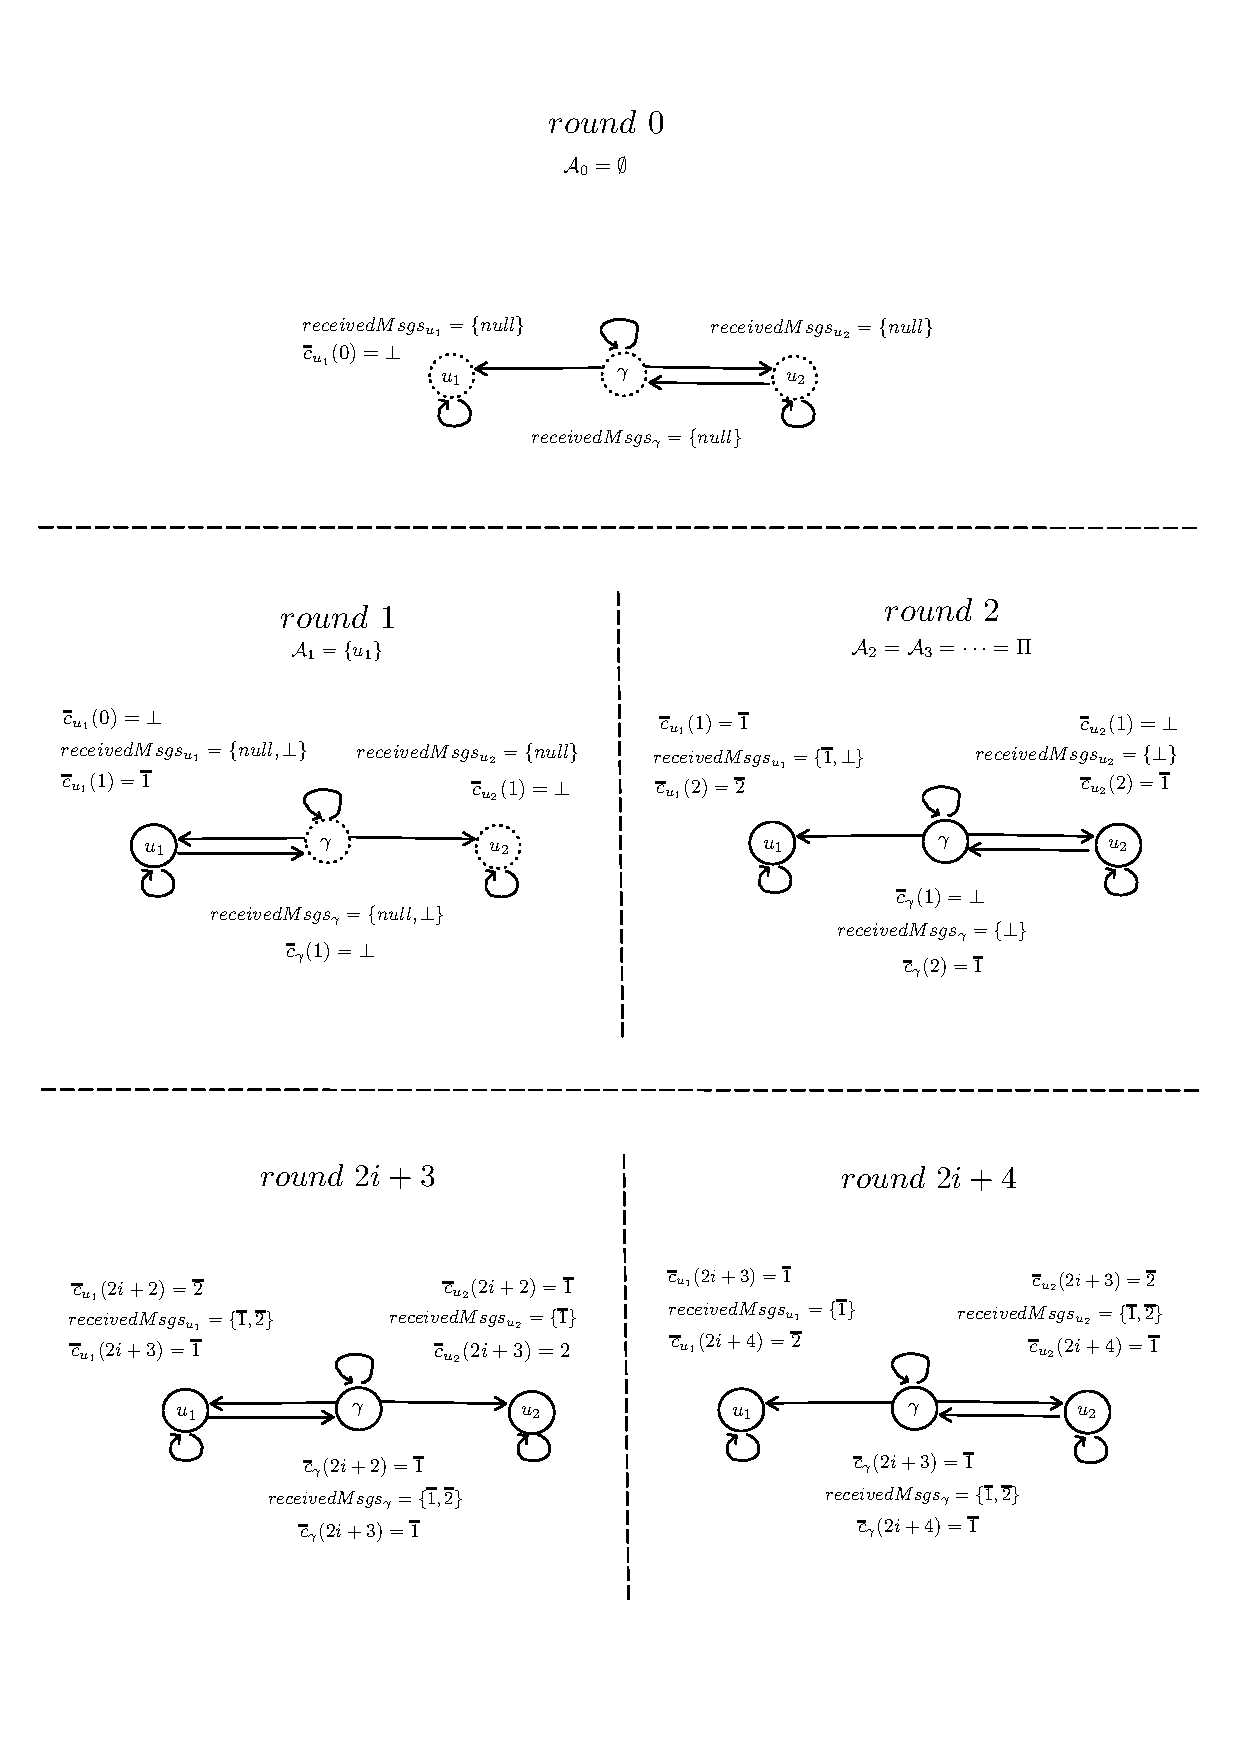
\includepdf[pages=-]{contre_exemple_k_2}

\section{$\mathrm{mod}\,k$-synchronization and coordinated algorithms}

Some algorithms like Paxos rely on the existence of a shared coordinator in each round.
A simple implementation consists in setting a rotating coordinator: 
each node holds the list of nodes. In the first round, the chosen coordinator is the first node in the list.
In the $i^{th}$ round, the chosen coordinator is the $i~mod~k^{th}$ node on the list.
This works out-of-the box when the starts are assumed to be synchronous.
However, when the starts are asynchronous, a prior $\mathrm{mod}\,n$-synchronization is required, where $n$ is the number of nodes in the shared list.
This is another typical use case of the \SM algorithm.

\section{Conclusion and future work}

As any complex reasoning by cases, the correctness proof  of the \SM   algorithm, 
	and more specifically the proof of the liveness property, is very error prone. 
This is a typical example of the relevance of formal verification for distributed algorithms. 
Indeed, in a later work~\cite{}, we used the interactive theorem prover Isabelle to encode the complete proof 
	of Theorem~\ref{thm:k>2}, and thus obtained a certificate for  \SM\!\!'s correctness when $k$ is greater than 2.
	
Since $\mathrm{mod}\,2$-synchronization is reducible to $\mathrm{mod}\,4$-synchronization,
	 our algorithm solves the $\mathrm{mod}\,k$-synchronization problem for any positive integer~$k$
	 in the class of  dynamic  graphs with a fixed center.
This class of dynamic graphs plays a crucial role regarding benign failures as it captures 
	the synchronous model with at most $n-1$ faulty senders, including the one with at most $n-1$ crashes.
In the wilder context of dynamic graphs, a natural question is whether the problem is still solvable 
	under weaker connectivity assumptions, in particular, in the class of dynamic graphs with a fixed root, 
	i.e., with a time-varying spanning tree at each round rooted at a fixed node.

\printbibliography

\section{Appendix: Non-uniform firing-squad algorithm}

The goal of this section is to provide an adaptation of the firing-squad algorithm to solve the relaxed problem called \textit{non-uniform synchronization}.
A subset $S \subseteq \Pi$ is the subset of correct nodes.
A correct node cannot crash, and any messages sent by $u \in S$ always reach its destination.
An incorrect node $u \in \Pi \setminus S$ which crashes in round $t$ must :
\begin{itemize}
	\item be correct until round $t-1$. All of its outgoing messages reach their destination.
	\item fail in round $t$ : only a subset of its outgoing messages reach their destination.
	\item be quiet in round $t+1$ and later.
\end{itemize}

We define the non-uniform synchronization problem as the conjunction of two properties:
\begin{description}
	\item[Safety:] If a correct node fires in round $t$, every correct node do so.
	\item[Liveness:] At least one correct node fires.
\end{description}

\noindent We define below the firing-squad algorithm adapted for a system with at most $f$ failures.
In this algorithm, each node maintains a counter. When every correct node is active, no node can receive a null message, and the nodes start incrementing their counters.
In the case where a node crashes in round $s^{max}$, there might be a discrepancy of one unit between the counter of the nodes.
This discrepancy might be preserved if a node crashes in round $s^{max}+1$.
However, the upper bond on the number of crash, and the sharing of counter values between nodes in each round guarantee that the counter values of every node will eventually be synchronized.

\begin{algorithm}[htb]\label{algo:code}
\begin{distribalgo}[1]
\BLANK \INDENT{\textbf{Initialization:}}
	\STATE $i_u \in \mathds{N}$, initially 0

\ENDINDENT \BLANK

\INDENT{\textbf{In each round $t$:}}
	\STATE send $i_u$ to all
	\STATE receive incoming messages
	\IF{no null received}
		\STATE $i_u \leftarrow 1+min~\{i_v(t-1), v \in HO(u,t)\}$ \label{line:union}
	\ELSE
		\STATE $i_u \leftarrow 0$
	\ENDIF
	\IF{$i_u \geq f+2$}
		\STATE fire
	\ENDIF
\ENDINDENT
\caption{The firing-squad algorithm} \label{algo:R}
\end{distribalgo}

\end{algorithm}

\subsection{Proof}

\begin{lemma} \label{lem:sync}
	If no node crash during a round $r \geq s^{max}$, every correct node must hold the same counter value.
\end{lemma}
\begin{proof}
	In such a round $r$, every correct node sends to all its counter.
	Since no crash happen, the remaining node stays quiet.
	Then, every node receive the same sets of values. The line \ref{line:union} guarantees that, at the end of the round, every node holds the same set.
\end{proof}

\begin{lemma} \label{lem:remain-synced}
	If at a round $r \geq s^{max}$, every correct node hold the same counter value, in every subsequent round, every node will hold the same counter value.
\end{lemma}
\begin{proof}
	This property can be proved by induction over the round number.
	Initially, we assume that every correct node hold the same counter value.
	In every subsequent round, the set of received values will be the same singleton for every node.
	Then, using the \ref{line:union}, the induction holds.
\end{proof}

\begin{theorem}
	The firing-squad algorithm solves the non-uniform synchronization problem if no node remains passive forever, and at most $f$ crash happen.
\end{theorem}
\begin{proof}
	If no node remains passive forever, $s^{max}$ is finite.
	\begin{description}
		\item[Safety:] Since at most $f$ crash may happen, there exists a round $r$ between $s^{max}$ and $s^{max}+f+1$ in which no crash happen.
			Then, using lemmas \ref{lem:sync} and \ref{lem:remain-synced}, we obtain that, in round $s^{max}+f+1$, every node holds the same counter value.
			Moreover, no node can reach $i_u \geq f+2$ before round $s^{max}+f+1$. 
			That proves safety.
		\item[Liveness:] Beyond round $s^{max}+1$, no node can receive a null message.
			We can prove that, in round $s^{max}+k$, the value $k$ is a lower bound of the counter values in the system.
			Thus, nodes must reach a counter value of $f+2$. That proves liveness.
	\end{description}
\end{proof}

\end{document}
